\begin{figure}[h]
    \centering
    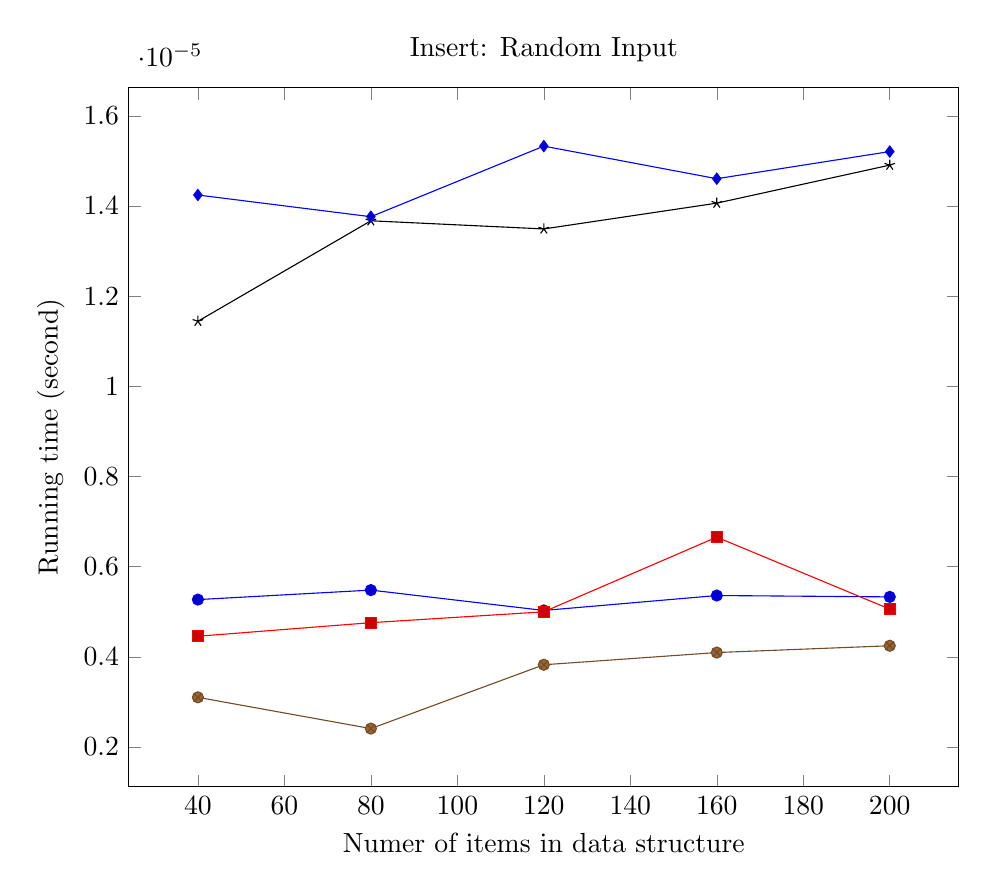
\begin{tikzpicture}
        \begin{axis}[
            xlabel={Numer of items in data structure},
            ylabel={Running time (second)},
            title={Insert: Random Input},
            width=\textwidth
        ]
		\addplot coordinates {
			(200, 5.330803460523726e-06)
			(160, 5.36092099423513e-06)
			(120, 5.029628123764951e-06)
			(80, 5.4813911290807486e-06)
			(40, 5.270568393100916e-06)
		};
		\addplot coordinates {
			(200, 5.059745657476355e-06)
			(160, 6.65597494204917e-06)
			(120, 4.999510590053547e-06)
			(80, 4.758570320717581e-06)
			(40, 4.4573949839588066e-06)
		};
		\addplot coordinates {
			(200, 4.246572247978974e-06)
			(160, 4.095984579777223e-06)
			(120, 3.824926776729854e-06)
			(80, 2.4094026940701953e-06)
			(40, 3.1021059683666865e-06)
		};
		\addplot coordinates {
			(200, 1.4908179169026426e-05)
			(160, 1.4064888226172912e-05)
			(120, 1.349265508672204e-05)
			(80, 1.3673360288279923e-05)
			(40, 1.1444662796833426e-05)
		};
		\addplot coordinates {
			(200, 1.52093545057852e-05)
			(160, 1.4607003832267651e-05)
			(120, 1.5329824640630817e-05)
			(80, 1.3763712889414137e-05)
			(40, 1.4245593428086068e-05)
		};
        \legend{}
        \end{axis}
    \end{tikzpicture}
    \caption{Average of 0 operations, benchmarked every 0, starting at 0.}
\end{figure}